\documentclass[letterpaper,12pt]{article}
\usepackage{array}
\usepackage{threeparttable}
\usepackage{fancyhdr,lastpage}
\pagestyle{fancy}
\lhead{}
\chead{}
\rhead{}
\lfoot{}
\cfoot{}
\rfoot{\footnotesize\textsl{Page \thepage\ of \pageref{LastPage}}}
\renewcommand\headrulewidth{0pt}
\renewcommand\footrulewidth{0pt}
\usepackage[format=hang,font=normalsize,labelfont=bf]{caption}
\usepackage{listings}
\lstset{frame=single,
  language=Python,
  showstringspaces=false,
  columns=flexible,
  basicstyle={\small\ttfamily},
  numbers=none,
  breaklines=true,
  breakatwhitespace=true
  tabsize=3
}

\usepackage{geometry}
\geometry{letterpaper,tmargin=1in,bmargin=1in,lmargin=1in,rmargin=1in}
%\renewcommand\headrulewidth{2pt}
%\renewcommand\footrulewidth{2pt}
\usepackage{amsmath}
\usepackage{amssymb}
\usepackage{amsthm}
\usepackage{mathtools}
\usepackage{pdflscape}
\usepackage{harvard}
\usepackage{setspace}
\usepackage{float,color}
%\usepackage{enumitem}
\usepackage[pdftex]{graphicx}
\usepackage{hyperref}
\hypersetup{colorlinks,linkcolor=red,urlcolor=blue}
\theoremstyle{definition}
\newtheorem{theorem}{Theorem}
\newtheorem{acknowledgement}[theorem]{Acknowledgement}
\newtheorem{algorithm}[theorem]{Algorithm}
\newtheorem{axiom}[theorem]{Axiom}
\newtheorem{case}[theorem]{Case}
\newtheorem{claim}[theorem]{Claim}
\newtheorem{conclusion}[theorem]{Conclusion}
\newtheorem{condition}[theorem]{Condition}
\newtheorem{conjecture}[theorem]{Conjecture}
\newtheorem{corollary}[theorem]{Corollary}
\newtheorem{criterion}[theorem]{Criterion}
\newtheorem{definition}[theorem]{Definition}
\newtheorem{derivation}{Derivation} % Number derivations on their own
\newtheorem{example}[theorem]{Example}
\newtheorem{exercise}[theorem]{Exercise}
\newtheorem{lemma}[theorem]{Lemma}
\newtheorem{notation}[theorem]{Notation}
\newtheorem{problem}[theorem]{Problem}
\newtheorem{proposition}{Proposition} % Number propositions on their own
\newtheorem{remark}[theorem]{Remark}
\newtheorem{solution}[theorem]{Solution}
\newtheorem{summary}[theorem]{Summary}
\numberwithin{equation}{section}
\bibliographystyle{aer}
\newcommand\ve{\varepsilon}
\newcommand\boldline{\arrayrulewidth{1pt}\hline}
\newcommand{\q}[1]{``#1''}

\def\changemargin#1#2{\list{}{\rightmargin#2\leftmargin#1}\item[]}
\let\endchangemargin=\endlist 

\usepackage{graphicx}
\graphicspath{ {images/} }

\usepackage{enumerate}
%\usepackage[shortlabels]{enumerate}
\setlength{\parindent}{24pt}
%\renewcommand{\baselinestretch}{2.0}
\usepackage{lipsum} % just for the example
\makeatletter
\newcommand{\verbatimfont}[1]{\renewcommand{\verbatim@font}{\ttfamily#1}}
\makeatother
%\usepackage{enumitem}
\usepackage{float}

\verbatimfont{\small}%


\begin{document}

\begin{flushleft}
   \textbf{\Large{Problem Set \#4}} \\
   MACSS 30100 \\
   Xinzhu Sun, 12147991\\
\end{flushleft}

\noindent \textbf{\large Problem 1}\par

\begin{enumerate} [\bfseries (a)]
\item The following graph is the histogram of the income distribution of the MACSS graduates:\\
\begin{figure}[H]
\centering
\fbox{\resizebox{4.75in}{3in}{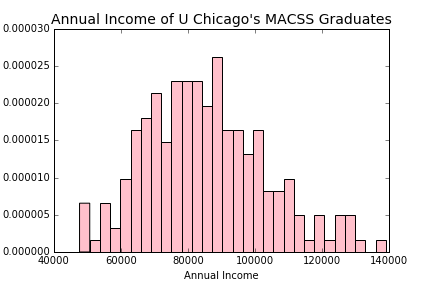
\includegraphics{Fig_1a}}}\
\end{figure}\par

\item The following graph is the lognormal PDF of GMM against the income distribution histogram of he MACSS graduates:
\begin{figure}[H]
\centering
\fbox{\resizebox{5in}{3in}{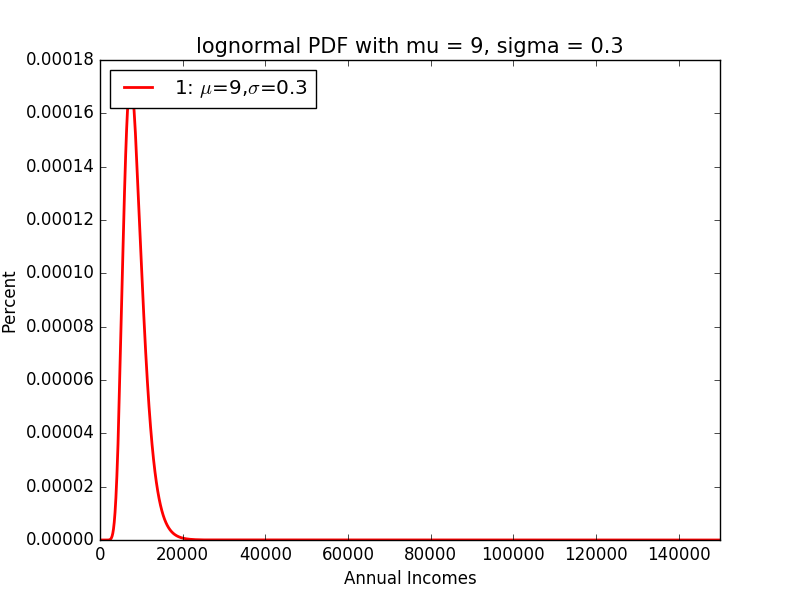
\includegraphics{Fig_1b}}}\
\end{figure}\par
The estimators of GMM are: \(\mu = 11.336910222, \, \sigma = 0.213027089137\). \\
The value of the GMM criterion function is \(1.84965511e-14\).\\
The data mean is 85276.8236063, the data standard deviation is  17992.542128.\\
The model mean is 85276.81387602663 ,the model standard deviation is 17992.5414622.\\
The two data moments and model moments of GMM are almost the same.\par	

\item The following graph is the lognormal PDF of two-step GMM against the income distribution histogram and the lognormal PDF of one-step GMM of the MACSS graduates:
\begin{figure}[H]
\centering
\fbox{\resizebox{5in}{3in}{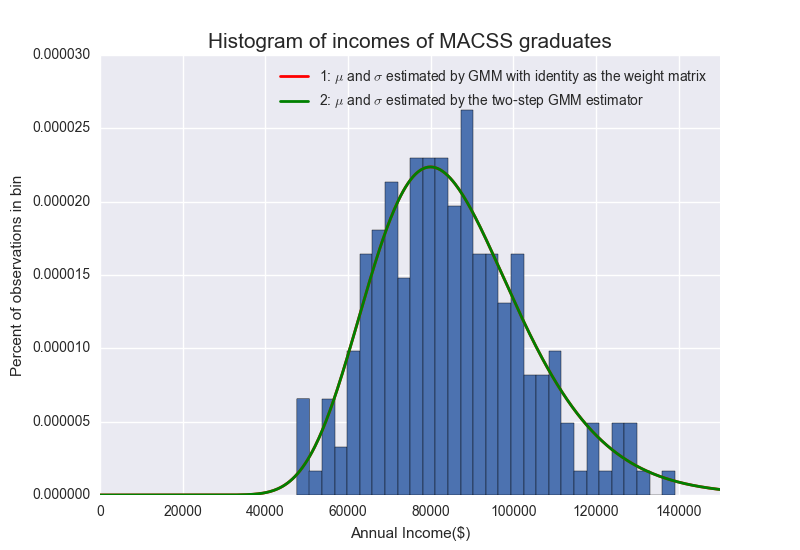
\includegraphics{Fig_1c}}}\
\end{figure}\par
The two-step GMM estimators are: \(\mu = 11.3369102322, \, \sigma = 0.213027115547\). \\
The value of the GMM criterion function is \(0.01225541\).\\
The data mean is 85276.8236063, the data standard deviation is 17992.542128.\\
The model mean is  85276.81463495447, the model standard deviation is 17992.5435696.\\
The two data moments and model moments of two-step GMM are almost the same.\par	

\item The following graph is the lognormal PDF of GMM with 3 moments against the income distribution histogram of the MACSS graduates:
\begin{figure}[H]
\centering
\fbox{\resizebox{5in}{3in}{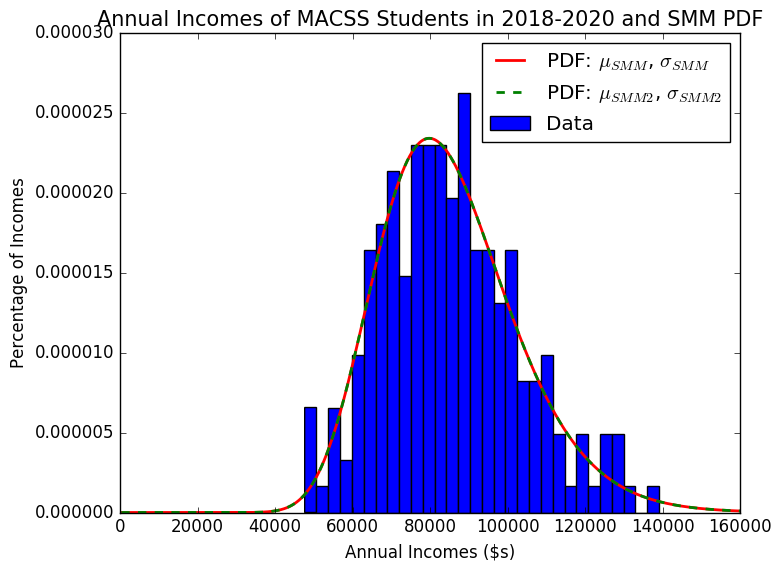
\includegraphics{Fig_1d}}}\
\end{figure}\par
The estimators of GMM with 3 moments are: \(\mu = 11.3356813276, \, \sigma = 0.210598453593\). \\
The value of the GMM with 3 moments criterion function is \(2.50777262e-11\).\\
The data moments are:\\
The proportion of students whose income is below \$75000 is: 0.3.\\
The proportion of students whose income is between \$75000 and \$100000 is: 0.5.\\
The proportion of students whose income is above \$100000 is: 0.2.\\
The model Moment are:\\
The proportion of students whose income is below \$75000 is: 0.30000000330502635. \\
The proportion of students whose income is between \$75000 and \$100000 is: 0.5000000061503362.\\
The proportion of students whose income is above \$100000 is: 0.1999999905446371.\\
The three data moments and model moments of GMM are almost the same.\par	

\item The following graph is the lognormal PDF of two-step GMM with 3 moments against the income distribution histogram and the lognormal PDF of one-step GMM with 3 moments of the MACSS graduates:
\begin{figure}[H]
\centering
\fbox{\resizebox{5in}{3in}{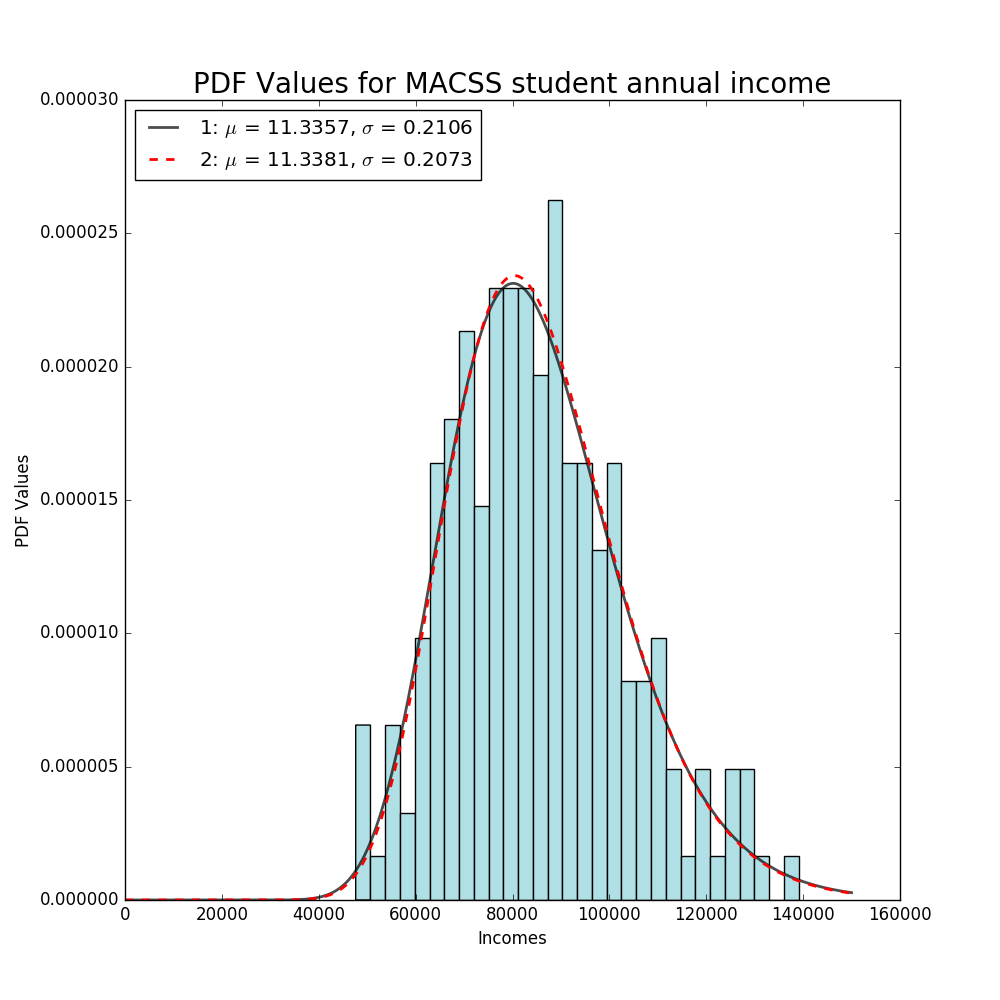
\includegraphics{Fig_1e}}}\
\end{figure}\par
The estimators of two-step GMM with 3 moments are: \(\mu = 11.3356813288 \, \sigma = 0.210598455913\). \\
The value of the two-step GMM with 3 moments criterion function is \(62.87294207\).\\
The data moments are:\\
The proportion of students whose income is below \$75000 is: 0.3.\\
The proportion of students whose income is between \$75000 and \$100000 is: 0.5.\\
The proportion of students whose income is above \$100000 is: 0.2.\\
The model Moment are:\\
The proportion of students whose income is below \$75000 is:  0.30000000329623505. \\
The proportion of students whose income is between \$75000 and \$100000 is: 0.5000000019381937.\\
The proportion of students whose income is above \$100000 is: 0.19999999476557095.\\
The three data moments and model moments of two-step GMM are almost the same.\par	

\item
Those four models are almost the same, cannot see any difference between them.\par
\end{enumerate}

\noindent \textbf{\large Problem 2}\par
The estimators are:\\
\begin{align*}
\beta_0 &= 0.25164486374\\
\beta_1 &= 0.0129334709799\\
\beta_2 &= 0.400500984533\\
\beta_3 &= -0.00999170971978\\
\end{align*}
The value of the criterion function is \(0.00182128980606\).


\end{document}